\chapter{Measuring distant objects with parallax}

%todo make two more telescopes on tripods, to have two setups going at a time. each group can use one telescope at a time, as long as scopes don't move.
%todo explain better in write-up what they are actually doing - maybe include conceptual tasks first, like the thumb demo and drawing objects, like in the lecture activity preview packet

\section{Introduction}

Since it takes time for light to travel to us from objects in the universe, the further out an object is, the further back in time we see it. So for us to have an accurate picture of how the universe was in the past, we need to know how far away things are. For things that are nearby on Earth, we can travel there and see how far we went, or how long we took to get there. For things further away like the moon, we can use Kepler's laws, or we can bounce a beam of light off of it and see how long it takes to get back. For objects outside of our solar system, it would take too long, and the light would disperse too much, for us to use this last technique. For those objects that are still relatively nearby, we can use the parallax technique as the first rung on our distance ladder.

\section{Procedure}

%Go out into the third floor hallway of KPTC (the long corridor near room 311).
Go to the fifth floor of Eckhardt Research Center. Near the elevators on the north side, there are
two telescopes%
% at the near end of the hallway, and an observing target is located at the far
end. The target is a mock-up of the night sky, but with colors and relative sizes of objects
greatly exaggerated to facilitate observations.

You will now use the telescope apparatus to measure the parallax of a “foreground star”
%(actually a ball on a stick)
(actually a nearby building), with the
%mock-up star field
Chicago skyline
serving as “background stars.”
%Place the “foreground star” part way down the hallway between the telescopes and the observing target.
Make sure that it is positioned so that sightlines from both telescopes
pass through both the “foreground star” and the “background stars,”
(an overlapping background of the skyline).
With your smartphone, take an image of the “foreground” and “background” stars through each telescope.
Also measure the distance between the two telescopes using a measuring tape and record
this value in your lab notebook. See Figure~\ref{par:fig:images} for example data.

\begin{figure}
	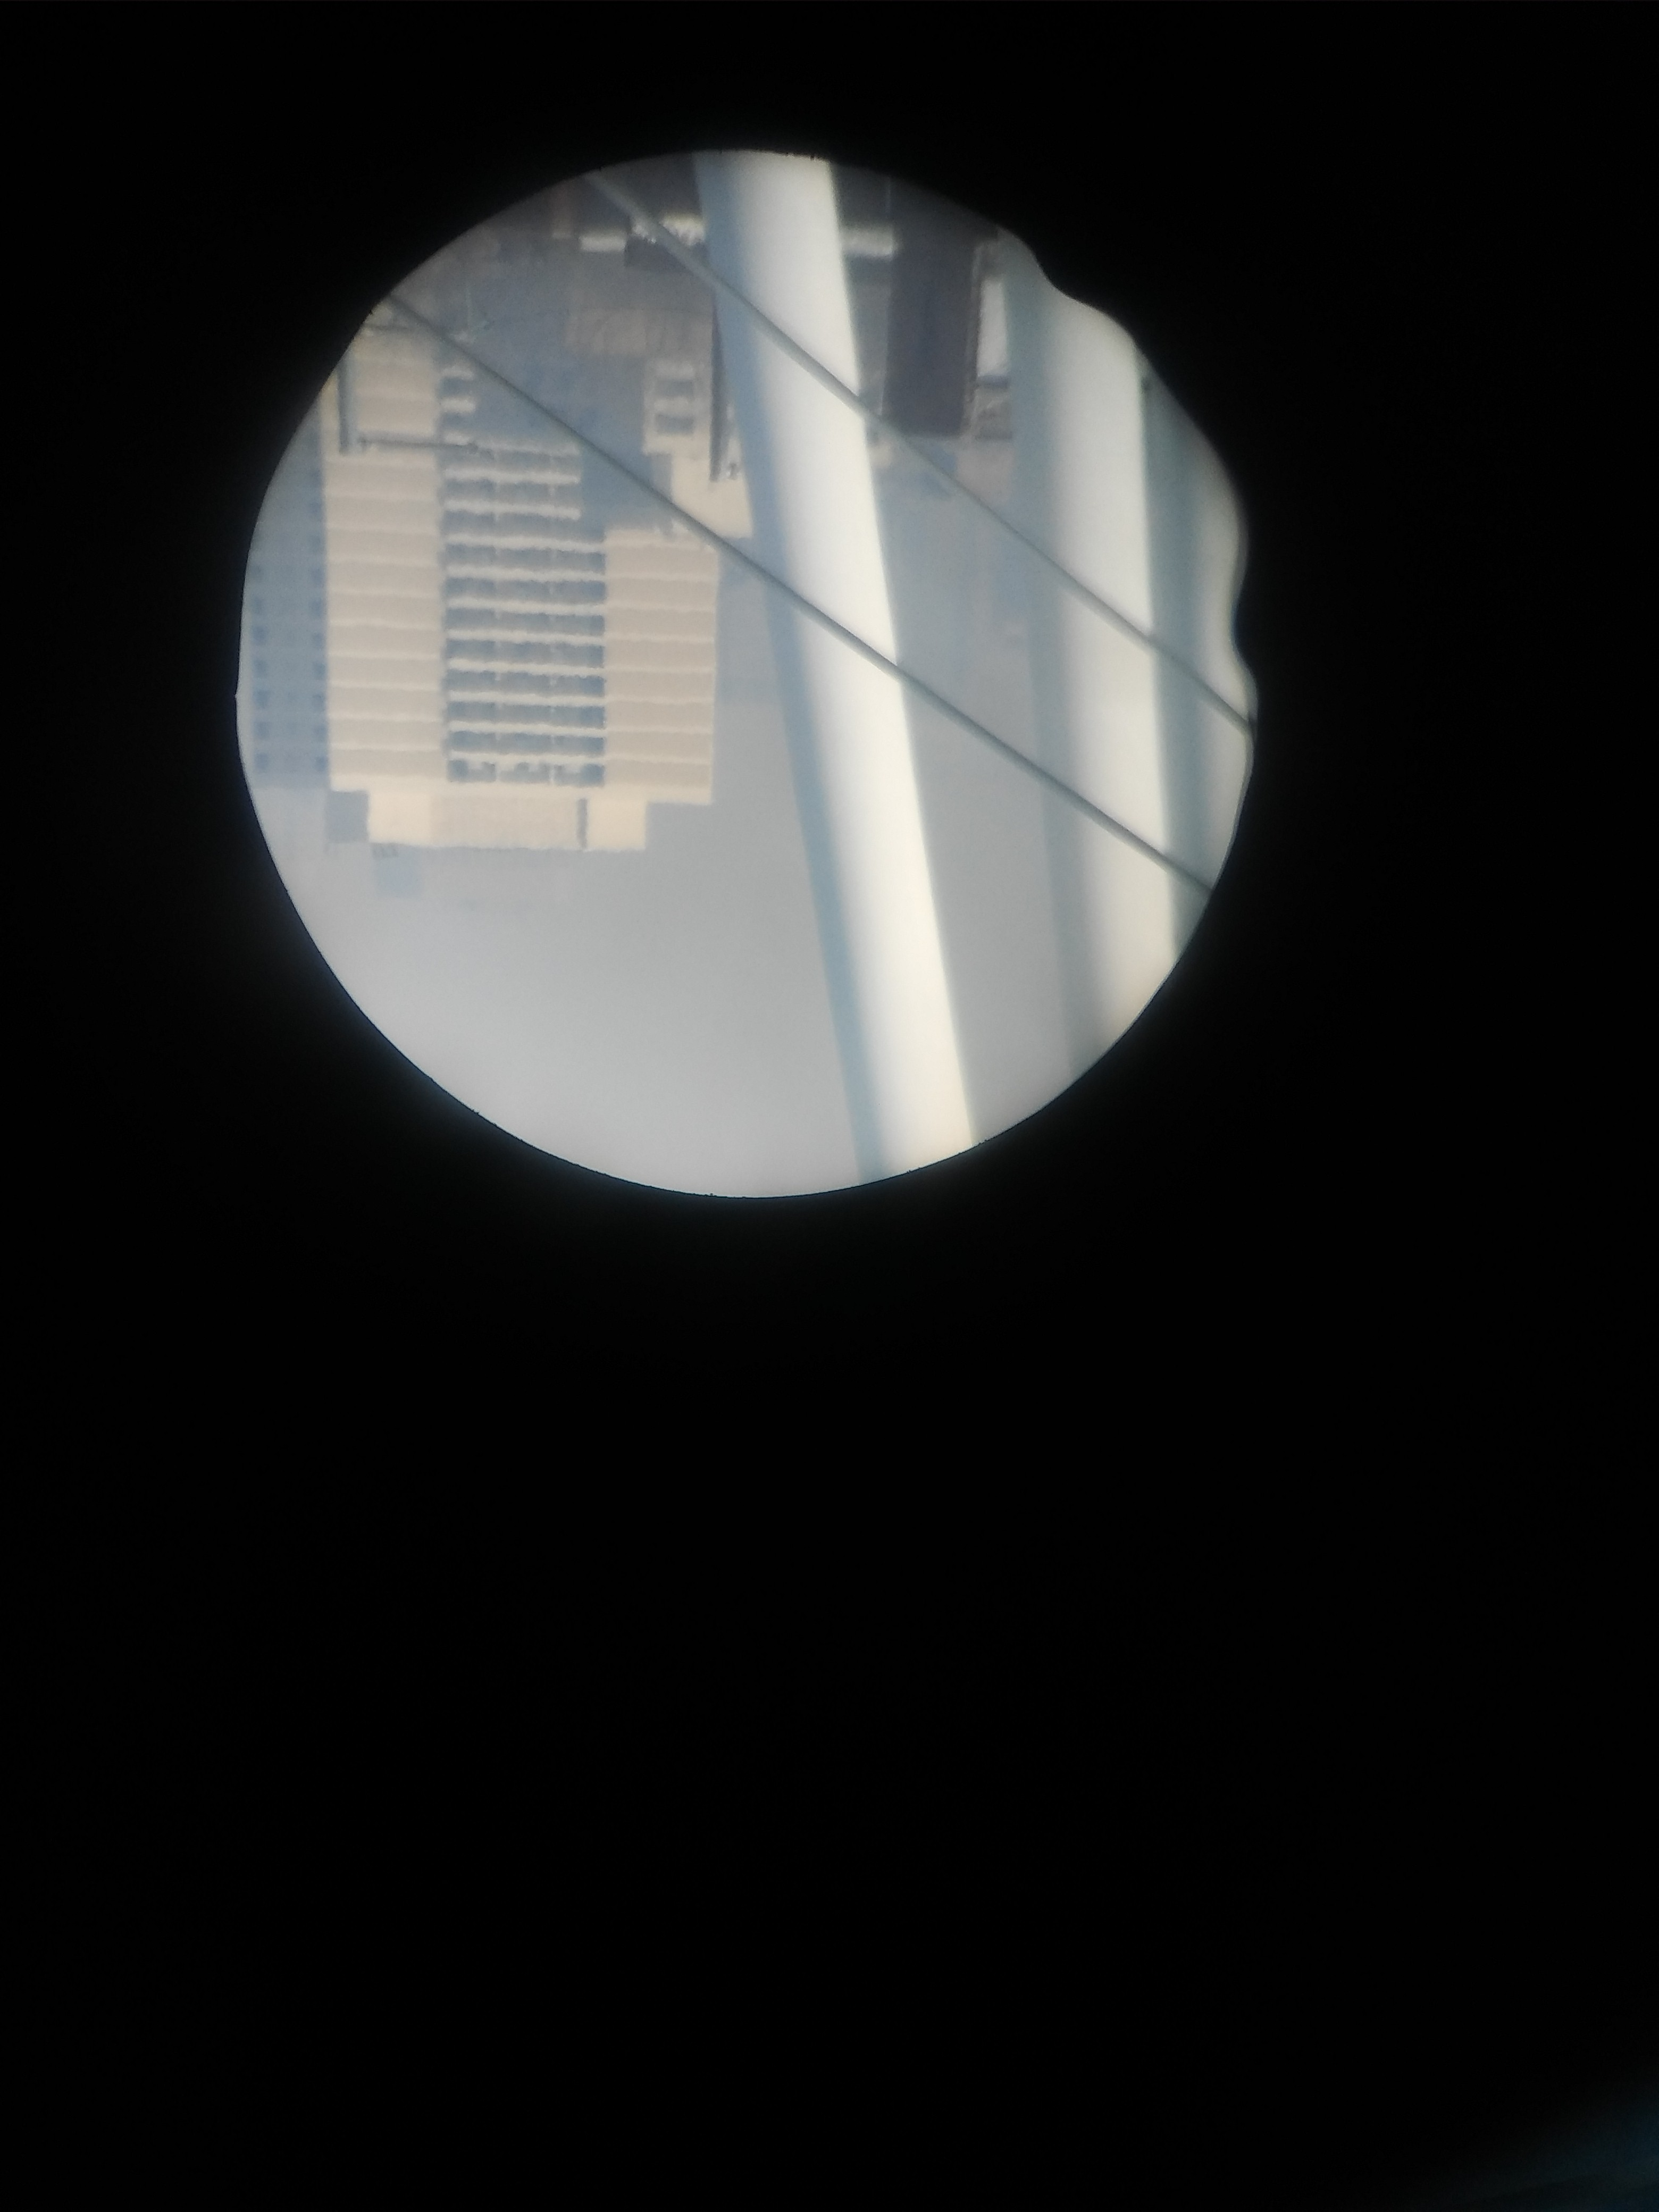
\includegraphics[width=0.5\textwidth]{parallax/parallax-image-1}
	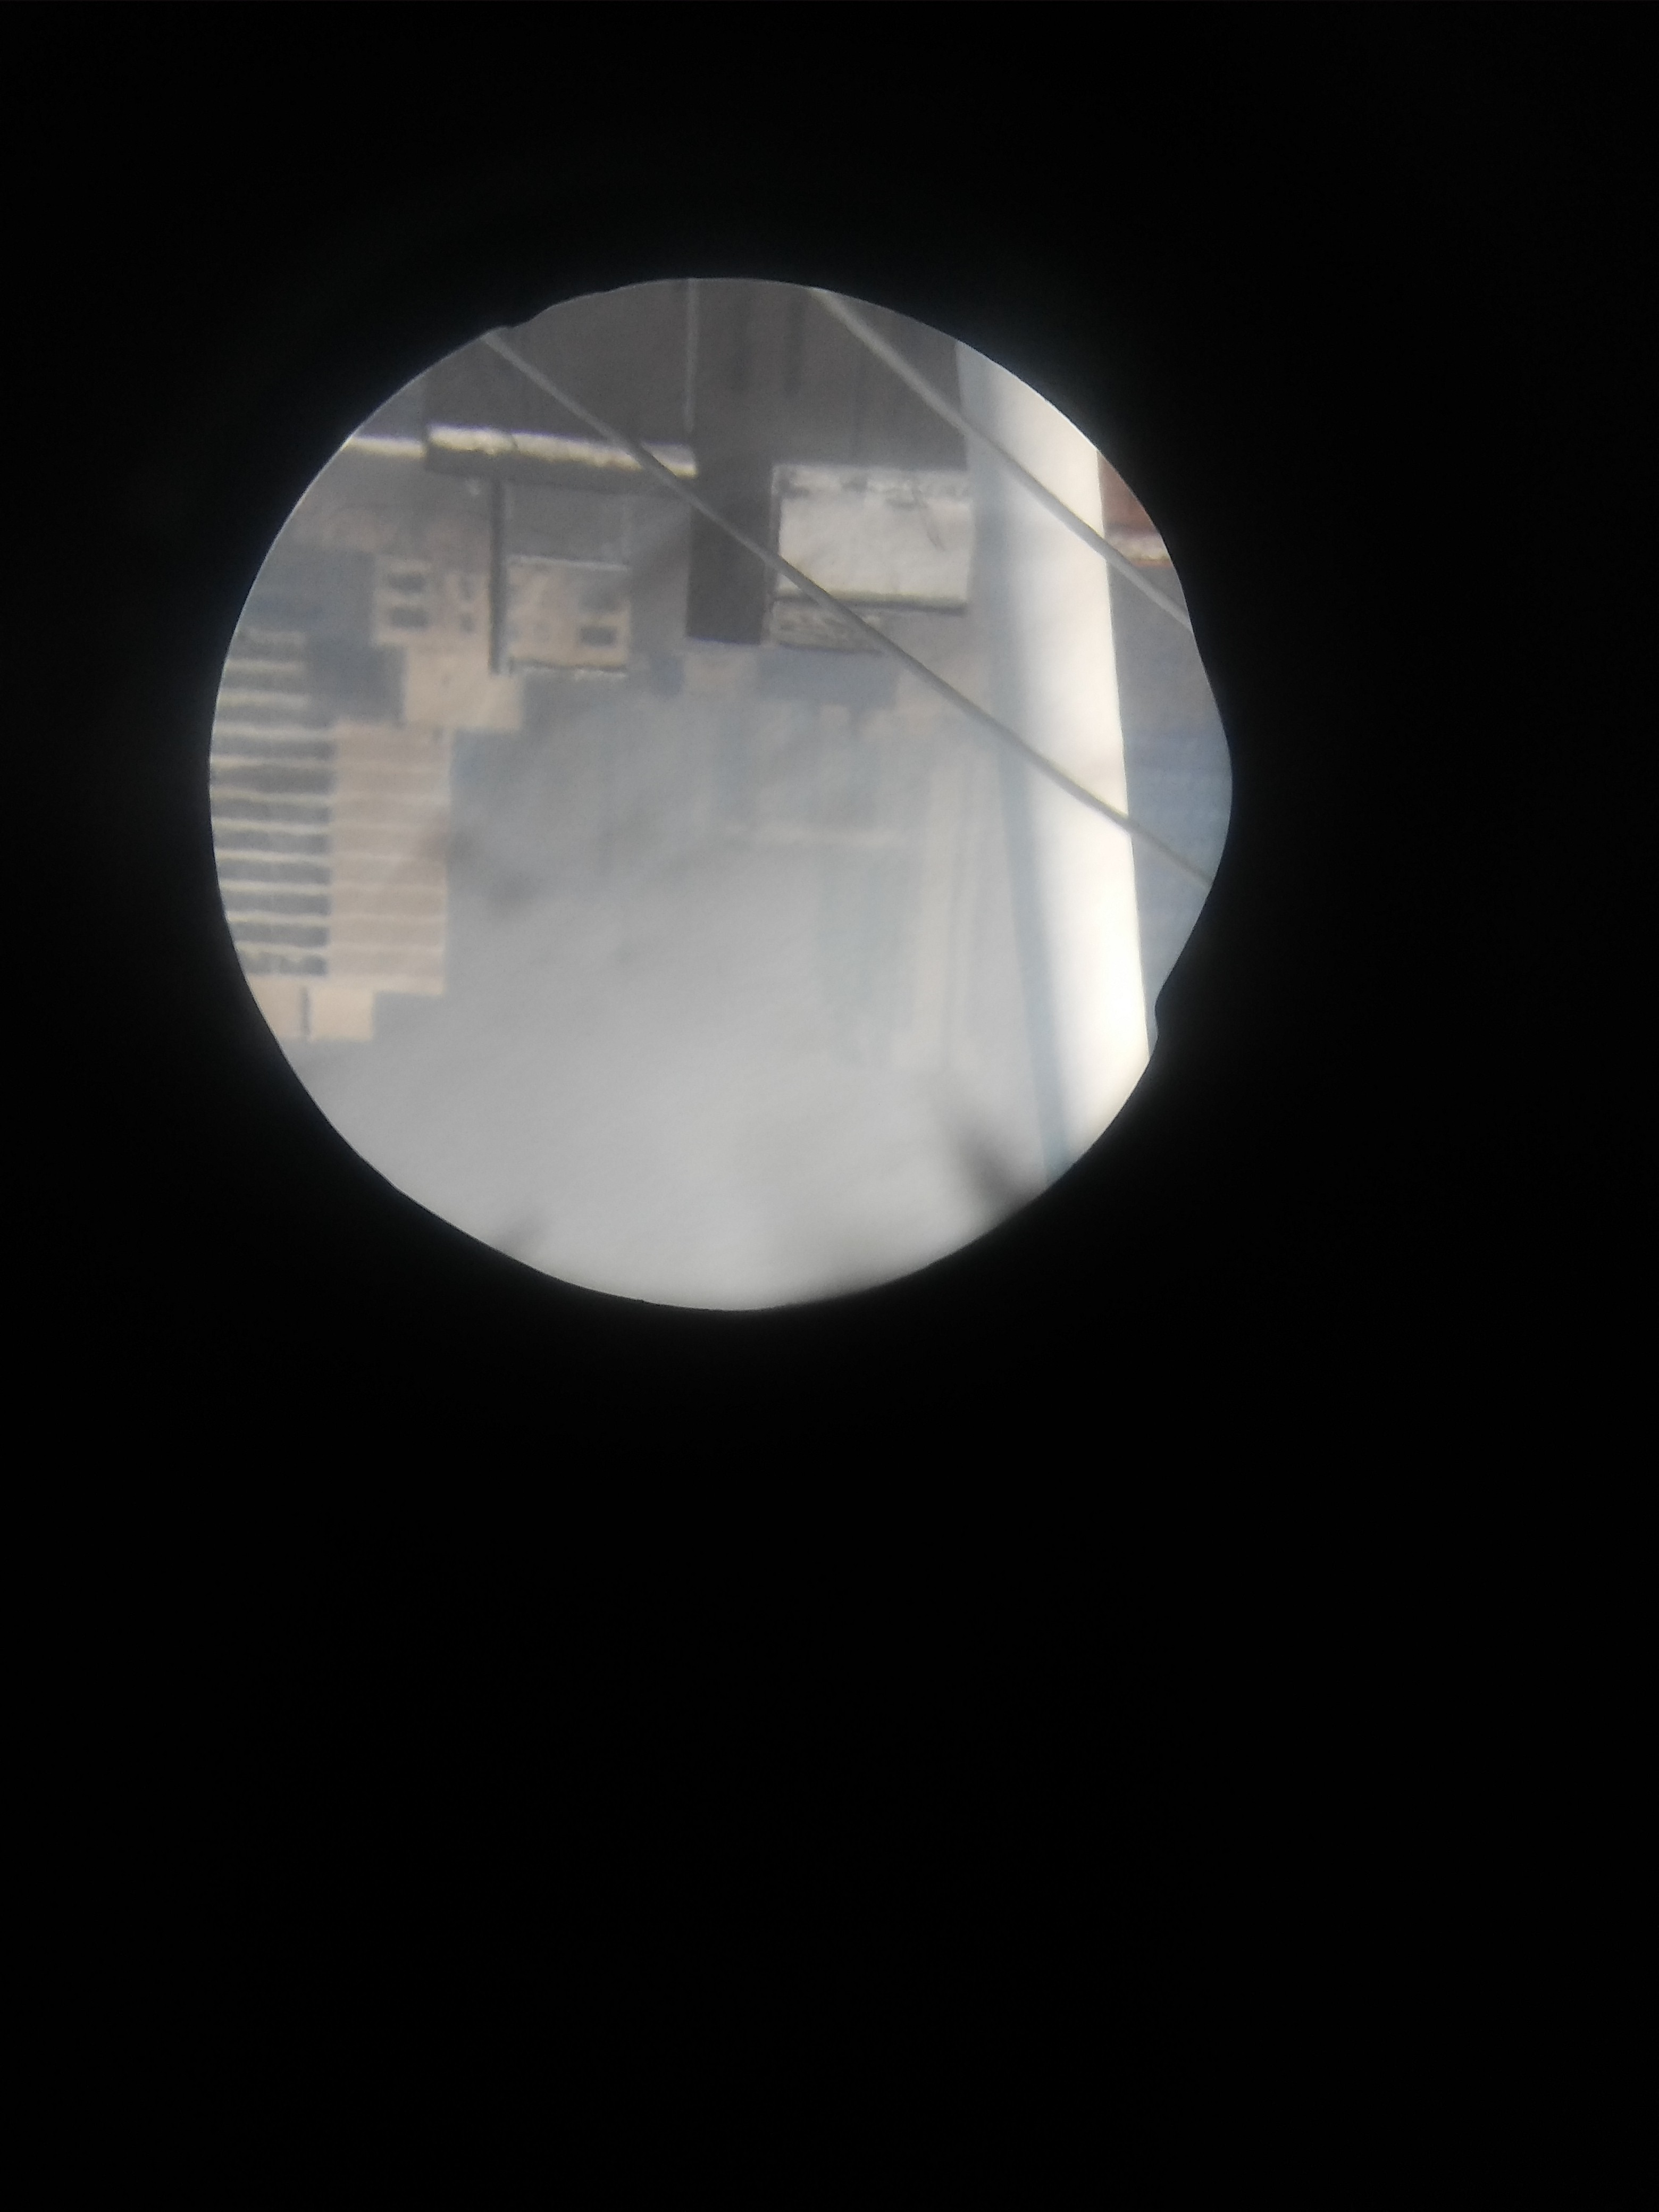
\includegraphics[width=0.5\textwidth]{parallax/parallax-image-2}
	\caption{Example images. My foreground ``star'' was the point defined by the left intersection of the lower cable and the white pillar on top of the gym on campus. One of my reference ``stars'' was the top right corner of the building in the background. Note that the images produced by this telescope are upside down.}\label{par:fig:images}
\end{figure}

You have now finished collecting data, so now it’s time to analyze it. Upload your
photographs to a computer. The simplest way to do this may be to email the images to
yourself from your phone. Give each file a descriptive name (e.g. ``\texttt{parallax\_left\_telescope}'').

You will now convert the images from their default format (likely .png or .jpeg) into .fits
files, a format commonly used by astronomers. This format will be readable by SAO
Image DS9, an astronomical image analysis tool. Open the first file in GIMP (“GNU
Image Manipulation Program”). From the FILE menu, select EXPORT AS, change the
file extension to “.fits,” and then click EXPORT. Repeat this procedure for each of your
images.

Open a saved .fits image of the star field in DS9. Your first task is to measure the size of
the field of view in pixels. Adjust the contrast so you can clearly see the field of view.
From the menu at the top of the screen, select REGION, SHAPE, LINE. On the first row
of buttons in the DS9 window, click EDIT then on the second row click REGION. Draw
a line across the field of view. On the first row of buttons, click REGION then on the
second row click INFORMATION. A window should pop up that will give you the length
of the line in physical units, that is, in pixels. Record this value in your lab notebook.

Now open the first parallax image. Measure the distance from the foreground star to
several reference background stars and record these values in your lab notebook. Make
sure to record both the X- and Y- offsets. Repeat these measurements for the second
parallax image using the same background stars.

\section{Calculations}

Given that the field of view of the Galileoscope is 1.5\textdegree
% (0.75\textdegree with the Barlow eyepiece)
calculate the \textit{plate scale} of your images, in arcsec/pixel.

Select a reference star from your parallax measurements. Using your plate scale,
determine the angular separation between the reference star and the target star. Record
the value for the total separation, $r$, and for both the horizontal ($x$) and vertical ($y$) components. You can
check your measurements against each other by inputting these values into the
Pythagorean formula: $r^2 = x^2 + y^2$. Do your measurements agree?

Repeat the above calculations for all reference stars in both of your parallax images. You
can now calculate the distance to the foreground star. The distance to a star using parallax
comes from simple trigonometry
\begin{equation}
 \tan p \approx p = \frac{a}{d},
\end{equation}
where we have made use of the small angle approximation $\sin(p) \approx p$. In this formula, $p$ is
the parallax angle in radians, $d$ is the distance to the star, and $a$ is half of the distance between the
two measurement positions. Figure~\ref{par:fig:figure} illustrates this geometry.

Therefore, $p$ is half the angular distance the target star appeared to move. To find that distance, for each reference star

\begin{figure}
	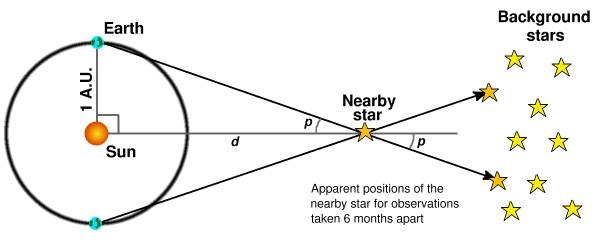
\includegraphics[width=\textwidth]{parallax/parallax-figure}
	\caption{Illustration of the geometry involved in a parallax measurement to determine $d$, the distance to a nearby star.}\label{par:fig:figure}
\end{figure}

Use each reference star to calculate an independent measurement of parallax. To do this, for each reference star, subtract the two displacement vectors from each other by components and find the magnitude of that difference vector. Divide by 2 and convert to radians to find $p$. After finding $p$ from each reference star, average these values together and estimate your uncertainty by finding the standard
deviation of these measurements. You can perform this calculations in Excel using the
functions AVERAGE() and STDEV(). Report your measurements in a table in your lab
report.

Also use a map to find the distance from you to your foreground star (with uncertainty). Compare these quantities with their uncertainties using the procedure found in Appendix~\ref{unc:sec:comparing}, to see the degree to which they agree.

\section{Questions}\label{par:sec:questions}

These should be included in your lab report.

\begin{enumerate}
	\item Your parallax measurements depend on an incorrect implicit assumption. What is
	this assumption, and how will it bias your results? How would you change the
	procedure in order to minimize this bias?
	\item How precise were your parallax measurements? What were the primary sources
	of uncertainty? How would you improve the procedure for future measurements?
\end{enumerate}

\section{Report checklist}

Include the following in your lab report. See Appendix~\ref{cha:lab-report-format} for formatting details. Each item below is worth 10 points, with an additional 10 points given for attendance and participation, for a total of 60 points for this lab.

\begin{itemize}
	\item A figure with your two images.
	\item The table of reference stars and displacement vectors.
	\item A statement of your final determined value of the distance, with uncertainty, and comparison with the distance found with a map. Show your work (see Appendix~\ref{cha:lab-report-format}).
	\item Answers to the questions in Section~\ref{par:sec:questions}, with justification.
	\item Your reflection on the experiment, as detailed in Appendix~\ref{cha:lab-report-format}.
\end{itemize}